\section * {\LARGE 2.Work Breakdown Structure}
\begin{center}
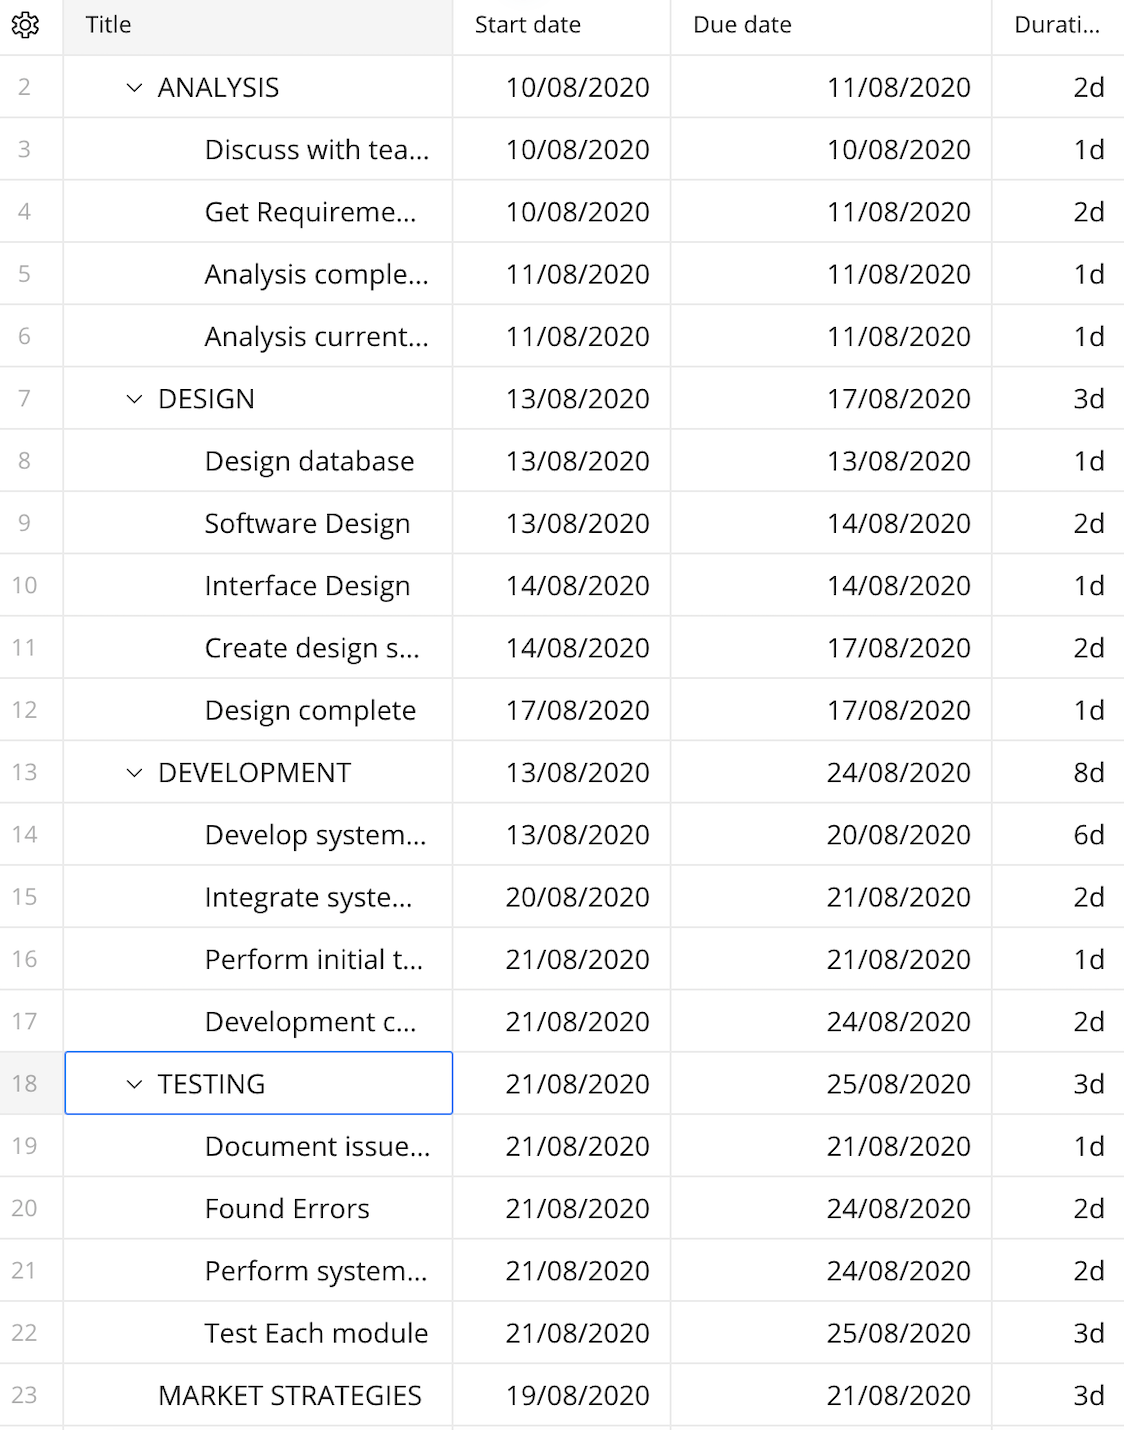
\includegraphics[scale=0.65]{FLOW.png}\\[0.75cm]
\end{center}



\begin{center}
\begin{tabular}{ l | r | r}

 Tasks & Completed by & Date  \\ 
 \hline \hline
 Analysis Phase & RAJWINDER KAUR & 11/AUG/2020  \\  
 Design Phase & RAJWINDER KAUR & 13/AUG-17/Aug  \\ 
 Development Phase & SANJEEV GUPTA & 11/AUG-24/AUG  \\
 Testing Phase & SANJEEV GUPTA & 21/AUG-25/AUG  \\ 
 Market strategies Phase & RAJWINDER KAUR & 19/AUG-21/Aug  \\ 
\end{tabular}
\end{center}

\section* {GIANTT CHART}
A Giantt chart, commonly used in project management, is one of the most popular and useful ways of showing activities (tasks or events) displayed against time. On the left of the chart is a list of the activities and along the top is a suitable time scale. Each activity is represented by a bar; the position and length of the bar reflects the start date, duration and end date of the activity.

\begin{center}
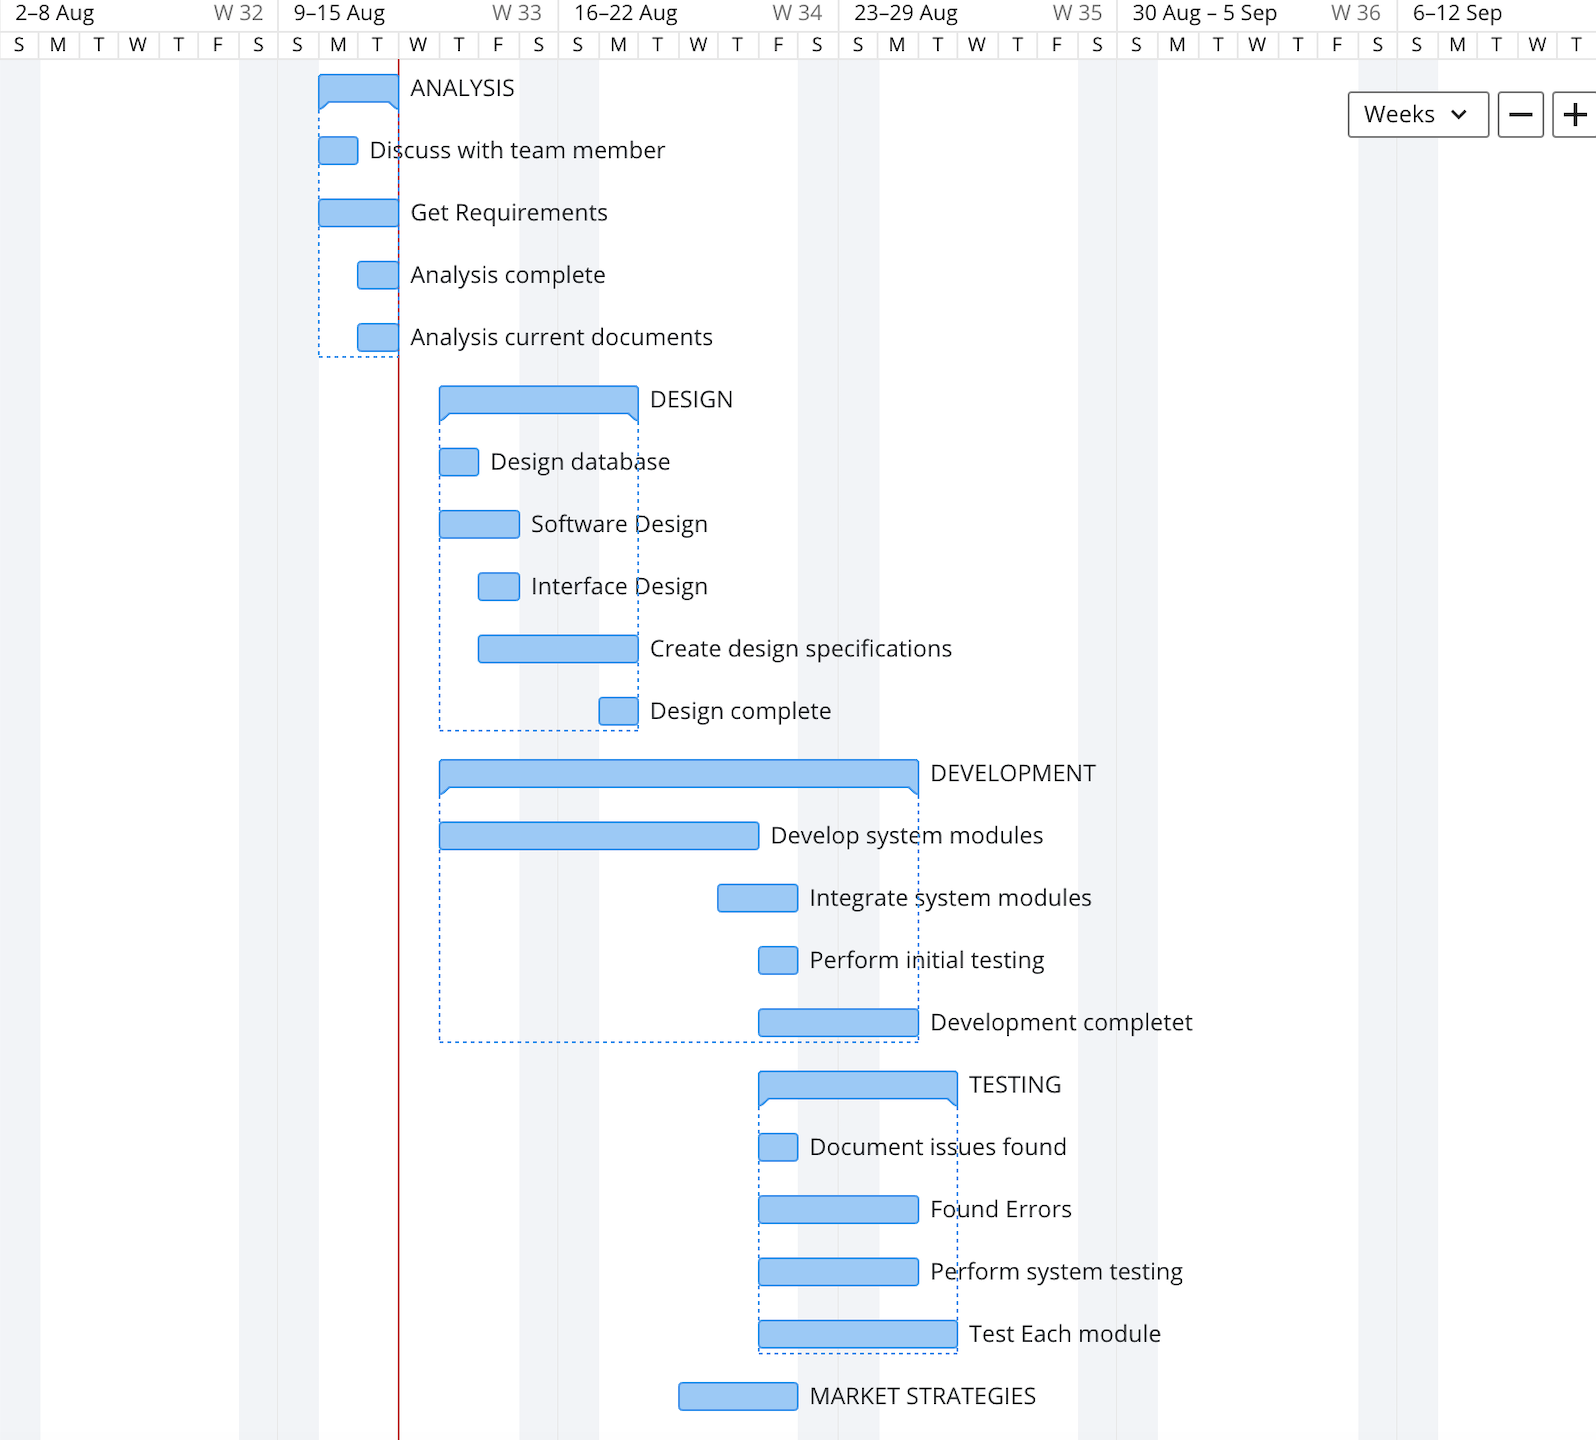
\includegraphics[scale=0.55]{GIANTT.png}\\[0.75cm]
\end{center}

\begin{center}
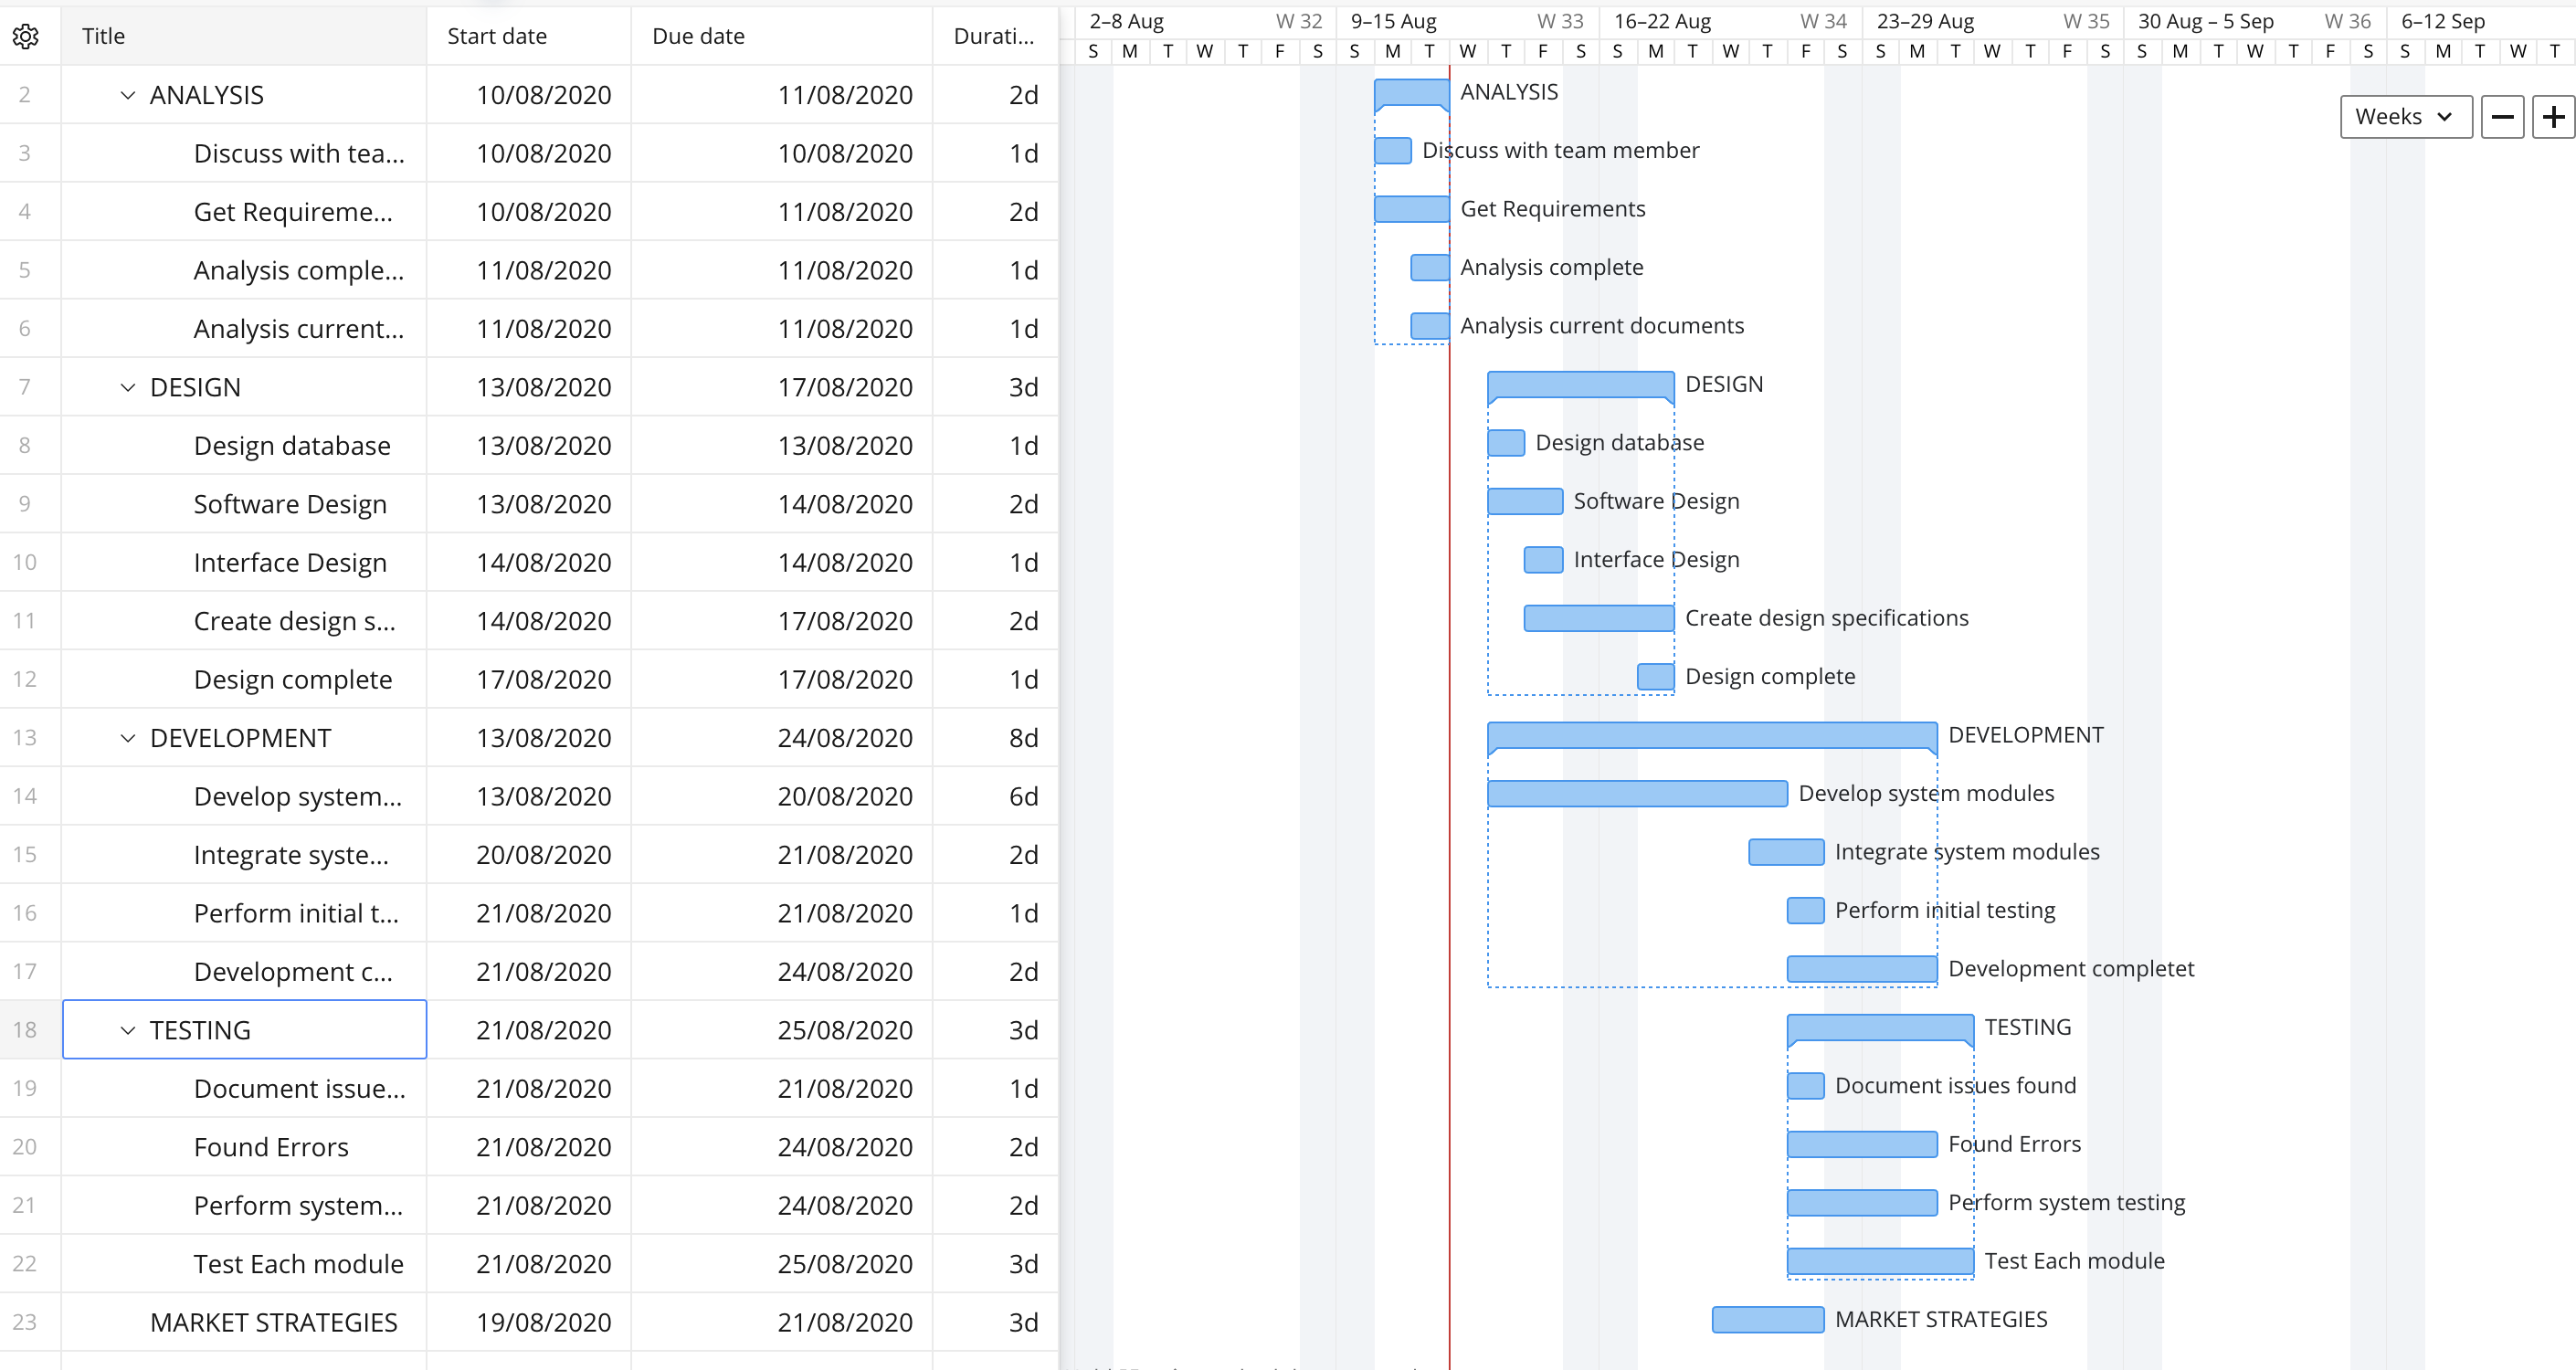
\includegraphics[scale=0.3]{CHART.png}\\[0.75cm]
\end{center}

\begin{enumerate}
    \item Work done by RAJWINDER KAUR C0764948
    \begin{verbatim}
    ANALYSIS, DESIGN AND MARKETTING STRATEGIES PHASE
    \end{verbatim}
    \item Work done by SANJEEV GUPTA C0761022
    \begin{verbatim}
    DEVELOPMENT AND TESTING PHASE
    \end{verbatim}
\end{enumerate}
